\documentclass[cjk,c,squeeze,shrink,dvipdfmx,12pt]{beamer}
% 以下は決まり文句
\usepackage{bxdpx-beamer}                      % dvipdfmx用の fix
\usepackage{pxjahyper}                         % 日本語で'しおり'
\usepackage{minijs}                            % min10ヤダ
\renewcommand{\kanjifamilydefault}{\gtdefault} % 既定をゴシック体に

\usetheme{KansaiDebian}
\usepackage{amsmath,amssymb,ulem}
\AtBeginSection[]{%
  \begin{frame}<beamer>\frametitle{本日のお品書き}\tableofcontents[currentsection]\end{frame}}

\title[Debian Updates \& Random Topics]{Debian Updates \& Random Topics}
\subtitle[OSC 2018 Hokkaido]{〜オープンソースカンファレンス 2018 Hokkaido〜}
\author[佐々木]{%
  佐々木洋平/Youhei SASAKI\\[1em]
  \href{mailto:uwabami@debian.or.jp}{uwabami@debian.or.jp}\\
  twitter/github: \textcolor{blue}{@uwabami}
}
\institute[Debian JP Project]{%
  {\footnotesize{%
      Debian JP Project/東京エリアDebian勉強会/関西Debian勉強会
    }}
}
\date[2018/07/07]{%
  {\tiny{2018年07月07日@札幌コンベンションセンター}}
}

\begin{document}
\setbeamercovered{transparent}
\takahashi[80]{ }
\takahashi[20]{例年より広い会場にビビってる. }
{%
  \setbeamertemplate{headline}{}
  \setbeamertemplate{footline}{}
  \begin{frame}
    \maketitle
  \end{frame}
}

\takahashi[70]{こんにちは}

\begin{frame}[fragile]
  \frametitle{Disclaimer}
  \begin{itemize}
  \item 疑問、質問、ツッコミ、茶々、\alert{大歓迎}
  \item その場でインタラクティブにどうぞ
  \item ハッシュタグ \alert{\#debianjp} で
  \end{itemize}
\end{frame}

\takahashi[70]{そんな\\こんなで}

\begin{frame}[fragile]{本日のお品書き}
  \tableofcontents
\end{frame}
%-------------------

\section{Debianとは? Debian JP とは?}
\takahashi[60]{Debianとは?}

\begin{frame}[fragile]{Debian とは?}

  \alert{フリー/オープン}な\alert{ユニバーサル}オペレーティングシステムを
  作成しようとするボランティアベースのプロジェクト。

  \vfill
  \centering
  \begin{tabular}{|c|c|c|}
    \hline
    ディストリ & 企業 & ボランティア \\ \hline
    RHEL & RedHat & なし  \\ \hline
    CentOS & RedHat & あり \\ \hline
    Ubuntu  & Canonical & あり \\ \hline
    \alert{Debian}  & \alert{なし} & \alert{あり} \\ \hline
  \end{tabular}
  \vfill
\end{frame}


\begin{frame}[fragile]{Debian とは?}
Linux カーネルだけではなく、FreeBSD や GNU/Hurd のカーネルを利用したOSも提供。

\centering
% ビルド前に画像を get しておくこと.
% \includegraphics[width=.2\paperwidth]{image201807-do/625px-NewTux.png}
% \includegraphics[width=.5\paperwidth]{image201807-do/523px-Freebsd_logo.png}
% \includegraphics[width=.2\paperwidth]{image201807-do/Hurd-logo.png}
\end{frame}


\begin{frame}[fragile]{Debian とは?}

  厳格/厳密なポリシーとガイドラインに沿った開発体制
  \begin{itemize}
  \item Debian 社会契約
  \item Debian フリーソフトウェアガイドライン
    \begin{itemize}
    \item オープンソースの定義の元
    \end{itemize}
  \item Debian Policy
  \end{itemize}

\end{frame}

\begin{frame}[fragile]{Debian とは?}
  \begin{columns}
    \begin{column}{.58\paperwidth}
      \begin{itemize}
      \item
        Ubuntu や Raspbian といったディストリビューションのベースとなっている
      \item
        Debian Derivatives(Debian 派生ディストリビューション)との協力体制の整備
      \end{itemize}
    \end{column}
    \begin{column}{.4\paperwidth}
      \centering
      % \includegraphics[height=.65\paperheight]{%
      %   image201807-do/500px-DebianFamilyTree1210.png}
    \end{column}
  \end{columns}
\end{frame}


\begin{frame}[fragile]{Debian とは?}
 世界規模で開発が行われており、63ヶ国、約1000名のDebian公式開発者が開発を行
 っている。パッケージメンテナや翻訳などの貢献者も入れるともっと多くの開発者が参加
 していることになる。

 \centering
 % \includegraphics[width=0.3\linewidth]{image201807-do/debconf_2015.jpg}
 % \includegraphics[width=0.3\linewidth]{image201807-do/debconf_2016.jpg}
 % \includegraphics[width=0.8\linewidth]{image201807-do/debconf_2017.jpg}
\end{frame}


\begin{frame}[fragile]{Debian とは?}
  2018年7月の時点で、
  \pause
  \begin{itemize}[<+->]
  \item
    最新版は {\alert{Debian 9.4}}, Stretch
  \item
    提供パッケージ数は{\alert{約51000}}
  \item
    公式にサポートするCPUアーキテクチャは{\alert{10}}
  \item {\alert{約2年毎}}にリリース
  \item next: Debian 10, Buster は2019年にリリース予定
  \item コードネームはトイ・ストーリーのキャラクターから
  \end{itemize}
\end{frame}

\begin{frame}[fragile]{Debian とは?: まとめ}
  \pause
  \begin{itemize}[<+->]
  \item Debianはフリー/オープンなOSを作成しようとするボランティアベースのプロジェクト。
  \item 自分たちの考えるフリーという言葉に関する定義、開発目的、パッケージングポリシーを厳格に決めている。
  \item 世界中に1000人以上の開発者がおり、他のディストリビューションのベースとして採用されている。
  \item 約2年毎にリリースが行われ、多くのパッケージとアーキテクチャをサポートしている。  \item 上記のような特徴から様々なところで利用されているLinuxディストリビューションである。
\end{itemize}
\end{frame}

%------------------
\begin{frame}[fragile]{Debian JP Project とは?\\[-.5em]{\normalsize{\texttt{https://www.debian.or.jp}}}}
  \pause
  \begin{itemize}[<+->]
  \item 日本でのDebianの普及を目的とした任意団体。
  \item %
    Debianの日本語による情報発信、
    ユーザとの情報交換、
    Debian 開発者、
    パッケージメンテナの育成など。
  \end{itemize}
\end{frame}


\begin{frame}
  \frametitle{Debian勉強会とは?%
    \\[-.5em]{\normalsize{\texttt{https://tokyodebian-team.pages.debian.net/}}}%
    \\[-.5em]{\normalsize{\texttt{https://wiki.debian.org/KansaiDebian}}}%
  }
  \pause
  \begin{itemize}[<+->]
  \item
    2005年1月開始, Debian Developer 上川さん発起人
  \item
    東京と関西で月に一回コンスタントに開催しているDebian開発者、
    ユーザによる勉強会。
  \item
    何がしたいのか?
    \begin{itemize}[<+->]
    \item
      MLとIRCで情報交換⇒face-to-faceであう場所がない
    \item
      まとまったドキュメントが出てこない
    \end{itemize}
  \item
    Debian勉強会でやっていること
    \begin{itemize}[<+->]
    \item
      定期的に集まる(場の提供)
    \item
      資料を作成して, 公開(GPL-2+) \\
      {\small \url{https://salsa.debian.org/tokyodebian-team/}}
    \end{itemize}
  \end{itemize}

\end{frame}

%-----------------------
\takahashi[40]{Any Questions?}

\section{Debian Updates}
\takahashi[60]{Debian Updates}

\begin{frame}[fragile]{%
    Debian Updates: Jessie%
    \\[-.5em]{\normalsize{Debian 8.x: oldstable}}
  }
  \pause
  \begin{itemize}[<+->]
  \item 2017/04/26: Debian 8.0 released
  \item[] :
  \item 2017/01/14: Updated Debian 8.7 released
  \item 2017/05/06: Updated Debian 8.8 released
  \item 2017/07/22: Updated Debian 8.9 released
  \item[] :
  \item \alert{2018/06/17: EOL}
  \item[←] oldstable のサポートは stable リリース後 1 年
  \item 2018/06/23: Updated Debian 8.11 released
  \item[※] LTS へ以降しました
  \end{itemize}
\end{frame}

\begin{frame}[fragile]{Debian Update: LTS%
    \\[-.5em]{\normalsize{Long Term Support}}
  }
  \pause
  \begin{itemize}[<+->]
  \item %
    LTSチームが\underline{利用企業からスポンサー支援を受け},
    i386, amd64, armelとarmhf のアーキテクチャに対して
    セキュリティアップデートを提供.
    期間は対象リリースのEOLから約2年間.
  \item %
    {\small{@see \href{https://wiki.debian.org/LTS}{https://wiki.debian.org/LTS}}}
  \item[※] %
    \alert{Debian 7.x: Wheezy の LTS は 2018/05/31 に終了しました}
    \begin{itemize}[<+->]
    \item 「Extended Long Term Support for Wheezy」というお話もあったり\\
      {\footnotesize{%
          \texttt{https://lists.debian.org/debian-devel/2018/02/msg00470.html}}}
    \end{itemize}
  \item %
    Debian 8.x: Jessie の LTS は 2020/06/30 まで提供の予定
    \begin{itemize}[<+->]
    \item 全てをカバーしている訳ではないことに注意!!
    \end{itemize}
  \end{itemize}
\end{frame}

\begin{frame}{Debian Update: Release Timetable}
  \pause
  \begin{itemize}[<+->]
  \item ``Bits from the release team: full steam ahead towards buster''
  \item Debian 10: Buster のリリースに向けたタイムラインが公開
    \begin{itemize}
    \item 2019-01-12 - Transition freeze
    \item 2019-02-12 - Soft-freeze
    \item 2019-03-12 - Full-freeze
    \end{itemize}
  \item Freeze とは?
  \end{itemize}
\end{frame}

{%
  \setbeamertemplate{headline}{}
  \setbeamertemplate{footline}{}
  \begin{frame}
    \includegraphics[width=\paperwidth]{./image201011/Debian-Release-Cycle01.png}
  \end{frame}
}
{%
  \setbeamertemplate{headline}{}
  \setbeamertemplate{footline}{}
  \begin{frame}
    \includegraphics[width=\paperwidth]{./image201011/Debian-Release-Cycle02.png}
  \end{frame}
}
{%
  \setbeamertemplate{headline}{}
  \setbeamertemplate{footline}{}
  \begin{frame}
    \includegraphics[width=\paperwidth]{./image201011/Debian-Release-Cycle03.png}
  \end{frame}
}
{%
  \setbeamertemplate{headline}{}
  \setbeamertemplate{footline}{}
  \begin{frame}
    \includegraphics[width=\paperwidth]{./image201011/Debian-Release-Cycle04.png}
  \end{frame}
}
{%
  \setbeamertemplate{headline}{}
  \setbeamertemplate{footline}{}
  \begin{frame}
    \includegraphics[width=\paperwidth]{./image201011/Debian-Release-Cycle05.png}
  \end{frame}
}

\begin{frame}{Debian Update: Release Timetable}
  \begin{itemize}
  \item ``Bits from the release team: full steam ahead towards buster''
  \item Debian 10: Buster のリリースに向けたタイムラインが公開
    \begin{itemize}
    \item 2019-01-12 - Transition freeze
    \item 2019-02-12 - Soft-freeze
    \item 2019-03-12 - Full-freeze
    \end{itemize}
  \item \alert{更新を入れたい場合には, 早めに作業しましょう/ご相談下さい.}
  \end{itemize}
\end{frame}

\begin{frame}{Debian Update: Call for Artwork}
  \pause
  \begin{itemize}[<+->]
  \item Call for Buster artwork proposals:\\
    \texttt{https://wiki.debian.org/DebianDesktop/Artwork/Buster}
    \begin{itemize}
    \item %
      \underline{2018/09/05: 投稿締切}
    \item %
      2018/09/06-09/25: レビュー期間
    \item %
      \underline{2018/09/26: 投票締切}
    \end{itemize}
  \item 興味のある方, 是非ご参加下さい!!
  \end{itemize}
\end{frame}


\begin{frame}[fragile]{Debian Update: Debconf}% [containsverbatim]
  \begin{itemize}
  \item 年に一回, Debian 開発者が集って開催するカンファレンス
  \item 今年は
    \alert{2018/07/29 - 08/05: Debconf18: 台湾 新竹市(Hsinchu)}
  \end{itemize}
  \begin{center}
%    \includegraphics[height=.4\textheight]{image201807-do/debconf18.png}
  \end{center}
  \begin{itemize}
  \item みなさん是非参加しましょう!!
  \end{itemize}
\end{frame}

\begin{frame}{Debian Update: その他の話題}
  \begin{itemize}
  \item ``its dead jim - alioth is gone''
    \begin{itemize}
    \item \texttt{debian-devel-announce/2018/06/msg00001.html}
    \item これまでソースコード開発などなどを提供していた alioth が停止 \\
      → \texttt{Gitlab on salsa.debian.org} へ移行
    \end{itemize}
  % \item \texttt{O: schroot -- Execute commands in a chroot environment}
  %   \begin{itemize}
  %   \item \texttt{BTS: \#900874}
  %   \item クリーンルーム環境を提供するパッケージをどうするか
  %   \item DebConf15 の会場で O されてるのどうすると話題になり、
  %     急遽 Raphael が引きとることになった→そろそろシンドイとの事.
  %   \end{itemize}
  \item Data Protection team delegation
    \begin{itemize}
    \item EU GDPR に関連したマネージメントを行なうチームができた
    \item \texttt{debian-devel-announce/2018/06/msg00000.html}
    \end{itemize}
  \end{itemize}
\end{frame}

\takahashi[70]{そんな\\こんなで}

\takahashi[40]{Any Questions?}

\section{日本語によるDebianの情報}
\takahashi[40]{日本語によるDebianの情報}

\begin{frame}[fragile]{日本語によるDebianの情報}
  \begin{itemize}
  \item Debian JP Project \\
    \url{http://www.debian.or.jp}
  \item 東京エリアDebian勉強会\\
    \url{http://tokyodebian.alioth.debian.org}
  \item 関西エリアDebian勉強会 \\
    \url{https://wiki.debian.org/KansaiDebianMeeting}
  \item Twitter \\
    \url{@debian_jp}
  \item slack
    \url{debian-jp.slack.com}
  % \item G+ コミュニティ \\
  %   \url{https://plus.google.com/u/0/communities/106942835439686570073}
  \end{itemize}
\end{frame}

\begin{frame}
  \frametitle{書籍情報}
  \begin{columns}
    \begin{column}{.5\paperwidth}
      \centering
      % \includegraphics[height=.6\paperheight]{image201807-do/SD201711.jpg}
    \end{column}
    \begin{column}{.5\paperwidth}
      \begin{itemize}
      \item %
        日本語での唯一の連載記事 \\
        「Debian Hot Topics」
      \end{itemize}
    \end{column}
  \end{columns}
\end{frame}

\begin{frame}
  \frametitle{書籍情報}
  \begin{columns}
    \begin{column}{.45\paperwidth}
      \centering
      % \includegraphics[height=.6\paperheight]{image201807-do/DebianHandbook.jpg}
    \end{column}
    \begin{column}{.54\paperwidth}
      \begin{itemize}
      \item %
        英語書籍の翻訳版
        \begin{itemize}
        \item %
          原版: The Debian Administrator's Handbook
          \begin{itemize}
          \item %
            Rapha\"el Hertzog, Roland Mas
          \item \url{https://debian-handbook.info/}
          \end{itemize}
        \end{itemize}
      \item %
        日本語で読める(現状)唯一の書籍!
      \item %
        パッケージ版:
        \texttt{debian-handbook}
      \end{itemize}
    \end{column}
  \end{columns}
\end{frame}

\takahashi[70]{そんな\\こんなで}

\begin{frame}[fragile]{Debian Update: Debconf%
  \\大事な事なので二回出します}% [containsverbatim]
  \begin{itemize}
  \item 年に一回, Debian 開発者が集って開催するカンファレンス
  \item 今年は
    \alert{2018/07/29 - 08/05: Debconf18: 台湾 新竹市(Hsinchu)}
  \end{itemize}
  \begin{center}
    % \includegraphics[height=.4\textheight]{image201807-do/debconf18.png}
  \end{center}
  \begin{itemize}
  \item \alert{みなさん是非参加しましょう!!}
  \end{itemize}
\end{frame}


\takahashi[40]{Any Questions?}
\takahashi[60]{Thanks!}

\end{document}
